\documentclass[10pt]{article}

\usepackage[margin=0.86in]{geometry}
\usepackage{amsmath,amssymb,amsfonts}
\usepackage{booktabs}
\usepackage{graphicx}
\usepackage{xcolor}
\usepackage{hyperref}
\usepackage{microtype}
\usepackage{caption}
\usepackage{subcaption}
\usepackage{array}
\usepackage{enumitem}
\usepackage{placeins}
\usepackage{xeCJK}
\setCJKmainfont{Noto Serif CJK JP}

\definecolor{linkblue}{HTML}{1D4ED8}
\definecolor{notebg}{HTML}{F8FAFC}
\definecolor{warnborder}{HTML}{D97706}

\hypersetup{
  colorlinks=true,
  linkcolor=linkblue,
  citecolor=linkblue,
  urlcolor=linkblue,
  pdftitle={[Fun Project] DeltaLoop-VLA and DeltaMem-pi0.5 v3 + CORM Technical Report},
  pdfauthor={DeltaLoop-VLA Research Project}
}

\setlength{\parskip}{0.40em}
\setlength{\parindent}{0pt}
\emergencystretch=2em

\title{\textbf{[Fun Project] DeltaLoop-VLA and DeltaMem-$\pi_{0.5}$ v3 + CORM:\\Multi-Timescale Gated DeltaNet Memory, Causal Object-Centric Reveal \& Transport, and Interference-Robust Readout on 16-Task \texttt{RoboMME}}}

\author{
  \textbf{[Fun Project] Technical Report} \\[0.2em]
  \small Repository: \href{https://github.com/k1000dai/deltanet-looped-vla}{\texttt{github.com/k1000dai/deltanet-looped-vla}} \\
  \small Project Page: \href{https://k1000dai.github.io/deltanet-looped-vla/}{\texttt{k1000dai.github.io/deltanet-looped-vla}}
}

\date{November 2026}

\begin{document}
\maketitle

\begin{abstract}
Long-horizon robotic manipulation under partial observability requires memory architectures that simultaneously track discrete state permutations, preserve fine 2D spatial landmarks across hundreds of demonstration frames, and remain stable across continuous multi-episode deployments without privileged human-issued memory resets. In this technical report, we present a three-phase empirical investigation spanning controlled synthetic benchmarks, a cached $450\text{M}$ \texttt{SmolVLA} backbone, and end-to-end $3.44\text{B}$ $\pi_{0.5}$ visuomotor policies on the 16-task \texttt{RoboMME} benchmark (\textbf{$0$ privileged or oracle test-time inputs}).
In \textbf{Phase 1 (\texttt{DeltaLoop-VLA})}, across $87$ synthetic runs and $10{,}720$ closed-loop rollouts, we establish a sharp mechanistic dissociation between \emph{expressive associative writing} ($\beta_t \in (0, 2)$ lifts $S_8$ swap tracking from $25.1\%$ to $100.0\%$) and \emph{weight-tied multi-hop readout} ($97.1\%$ ID / $80.4\%$ OOD pointer chasing), showing via linear probes that a $520\text{ KB}$ 2-layer \texttt{fp32} Gated DeltaNet retains $93.52\%$ of counts and $4.36\text{ px}$ coordinates despite frozen \texttt{SmolVLA}'s $<10\%$ motor ceiling.
In \textbf{Phase 2 (\texttt{DeltaMem-$\pi_{0.5}$})}, scaling \texttt{Hybrid\allowbreak Surprise\allowbreak GDNBridge} + \texttt{Episode\allowbreak Boundary\allowbreak ForgetGate} + \texttt{Stage-C Hop-2} to $3.44\text{B}$ $\pi_{0.5}$ achieves $48.75\%$ single-session and $41.67\%$ un-reset $k=3$ success on \texttt{test240} ($+26.25\text{ pp}$ over \texttt{FrameSamp+Modulator}'s $15.42\%$, $p_{\mathrm{McN}} = 1.16 \times 10^{-14}$), while exposing a reveal-inversion singularity ($\|\mathbf{F}_t - \mathbf{F}_0\|_2 = 0$) and container-swap transport bottleneck behind its $-8.08\text{ pp}$ gap to \texttt{T\textsuperscript{2}Mem} ($56.83\%$).
In \textbf{Phase 3 (\texttt{DeltaMem-$\pi_{0.5}$ v3 + CORM})}, introducing \emph{Causal Object-Centric Reveal \& Transport Memory} (\texttt{CORM}) alongside shared-VLM \texttt{DeltaGround-VLM} and proprioceptive transition guards (\texttt{ReFINE}-inspired action-transition alignment \cite{hong2026refine}) clears a pre-registered $240$-episode validation gate at \textbf{$73.33\%$} and achieves \textbf{$71.00\%$ ($568/800$, 95\% CI $[67.72\%, 74.12\%]$)} on the full official held-out \texttt{RoboMME} \texttt{test} split (\textbf{$69.29\%$} on the $560$ completely untouched \texttt{ep 15..49} episodes), \textbf{surpassing published \texttt{T\textsuperscript{2}Mem} ($56.83\%$) by $+14.17\text{ pp}$ ($p_{\mathrm{binom}} = 1.86 \times 10^{-16}$, task-stratified two-sample $p = 3.94 \times 10^{-19}$)} at $410.6\text{ ms/chunk}$ and $3.04\text{ MiB}$ episode fast state ($12\times$ smaller than \texttt{T\textsuperscript{2}Mem}), while retaining \textbf{$70.83\%$ ($170/240$)} under un-reset $k=3$ cross-session interference ($+55.42\text{ pp}$, $4.59\times$ over \texttt{FrameSamp+Modulator}, $p_{\mathrm{McN}} = 1.09 \times 10^{-37}$).
\end{abstract}

% =============================================================================
\section{Introduction and Problem Setting}
% =============================================================================
Standard Vision-Language-Action (VLA) policies condition action generation almost exclusively on the current camera frame and static language prompt \cite{pi05_2025,smolvla2025}, rendering them effectively Markovian. On non-Markovian manipulation suites such as \texttt{RoboMME} \cite{mmevla2026}---which evaluates $16$ ManiSkill3 tabletop tasks across \texttt{Counting}, \texttt{Permanence}, \texttt{Reference}, and \texttt{Imitation}---memoryless $\pi_{0.5}$ achieves only $17.93\%$ published macro-average success ($21.67\%$ in our PyTorch reproduction). Existing embodied memory approaches face an acute trilemma:
\begin{enumerate}[leftmargin=1.6em,nosep]
  \item \textbf{Explicit token buffers (\texttt{FrameSamp+Modulator} \cite{mmevla2026}, $44.51\%$):} Uniformly subsampling $32$ past frames ($512$ tokens, $4.0\text{ MiB}$) drops brief occlusion-reveal flashes and \textbf{collapses catastrophically when deployed across continuous multi-episode streams without oracle \texttt{reset()} calls} \cite{robommeinterf2026} ($45.83\% \to 15.42\%$ in our held-out $k=3$ test).
  \item \textbf{External VLM keyframe reasoners (\texttt{MemER} \cite{mmevla2026}, $42.38\%$):} Autoregressive VLM subgoal decoding incurs $10{,}135\text{ ms/chunk}$ latency ($<0.1\text{ Hz}$) and fails on fine motion imitation ($29.50\%$) and reactive timing (\texttt{StopCube} $0.00\%$).
  \item \textbf{Heavy per-layer MLP fast weights (\texttt{T\textsuperscript{2}Mem} \cite{t2mem2026}, $56.83\%$):} Maintaining $18 \times 16$ per-head GeLU MLPs requires $36.35\text{ MiB}$ of fast state per episode, $1{,}536\text{ H200}$ GPU-hours of alternating second-order JVP/secant training, lacks an exponential forget gate for un-reset multi-session streaming, and struggles severely on container swaps (\texttt{Button\allowbreak Unmask\allowbreak Swap} $20.00\%$, \texttt{Video\allowbreak Unmask\allowbreak Swap} $29.33\%$) and long-horizon spatial reference (\texttt{Video\allowbreak Place\allowbreak Order} $30.00\%$, \texttt{Video\allowbreak Place\allowbreak Button} $35.33\%$).
\end{enumerate}

This report chronicles our complete three-phase progression combining $O(1)$ linear-recurrent associative state (\texttt{Gated DeltaNet} \cite{yang2025gdn,grazzi2025unlocking}), non-privileged surprise landmarks \cite{behrouz2025titans}, shared-VLM stage grounding, action-transition alignment \cite{hong2026refine}, and causal object-centric reveal \& transport memory (\texttt{CORM}) to surpass \texttt{T\textsuperscript{2}Mem} with decisive statistical significance under zero test-time privileged inputs.

% =============================================================================
\section{Phase 1: Mechanistic Dissociation of Writing and Multi-Hop Readout}
% =============================================================================
Phase 1 (\texttt{DeltaLoop-VLA}) isolated when expressive state writing versus iterative multi-hop readout is mathematically necessary across $87$ shortcut-audited synthetic runs ($3$ seeds) and $10{,}720$ closed-loop \texttt{RoboMME} rollouts on scratch ($28\text{M}$--$40\text{M}$) and cached $450\text{M}$ \texttt{lerobot/smolvla\_base} \cite{smolvla2025} backbones. Our recurrent core updates a matrix state $\mathbf{S}_u^{(h)} \in \mathbb{R}^{d_v \times d_k}$ via a motion-gated Gated DeltaNet transition with expanded step size $\beta_u^{(h)} \in (0, 2)$ \cite{grazzi2025unlocking}:
\begin{equation}
  \mathbf{S}_u^{(h)} = \exp\!\big(g_u^{(h)}\big)\!\left(\mathbf{I} - \beta_u^{(h)}\mathbf{k}_u^{(h)}{\mathbf{k}_u^{(h)}}^\top\right)\mathbf{S}_{u-1}^{(h)} + \beta_u^{(h)}\mathbf{v}_u^{(h)}{\mathbf{k}_u^{(h)}}^\top, \qquad \beta_u^{(h)} \in (0, 2), \; g_u^{(h)} \le 0.
  \label{eq:gdn}
\end{equation}
At $\beta_u^{(h)} \to 2$, the Householder factor $(\mathbf{I} - 2\mathbf{k}\mathbf{k}^\top)$ carries eigenvalue $-1$ along $\mathbf{k}$, lifting 1-layer $S_8$ swap tracking from $25.1\%$ ($\beta \in (0,1)$) to \textbf{$100.0 \pm 0.0\%$} both in-distribution and OOD ($k=5,6$), whereas retroactive pointer chasing (\texttt{Task 1A-Retro}) requires weight-tied \texttt{Prelude--Core--Coda} multi-hop readout (\textbf{$94.8\%$--$97.1\%$ ID}, \textbf{$76.4\%$--$80.4\%$ OOD}). Crucially, linear probes on frozen $520\text{ KB}$ GDN states (Figure~\ref{fig:phase1}b) verified \textbf{$93.52\%$ count retention} and \textbf{$4.36\text{ px}$ target localization}, proving that cached \texttt{SmolVLA}'s $<10\%$ success stemmed from frozen $8\times 8$ visuomotor actuation rather than memory capacity.

\begin{figure}[t]
  \centering
  \begin{subfigure}[t]{0.49\textwidth}
    \centering
    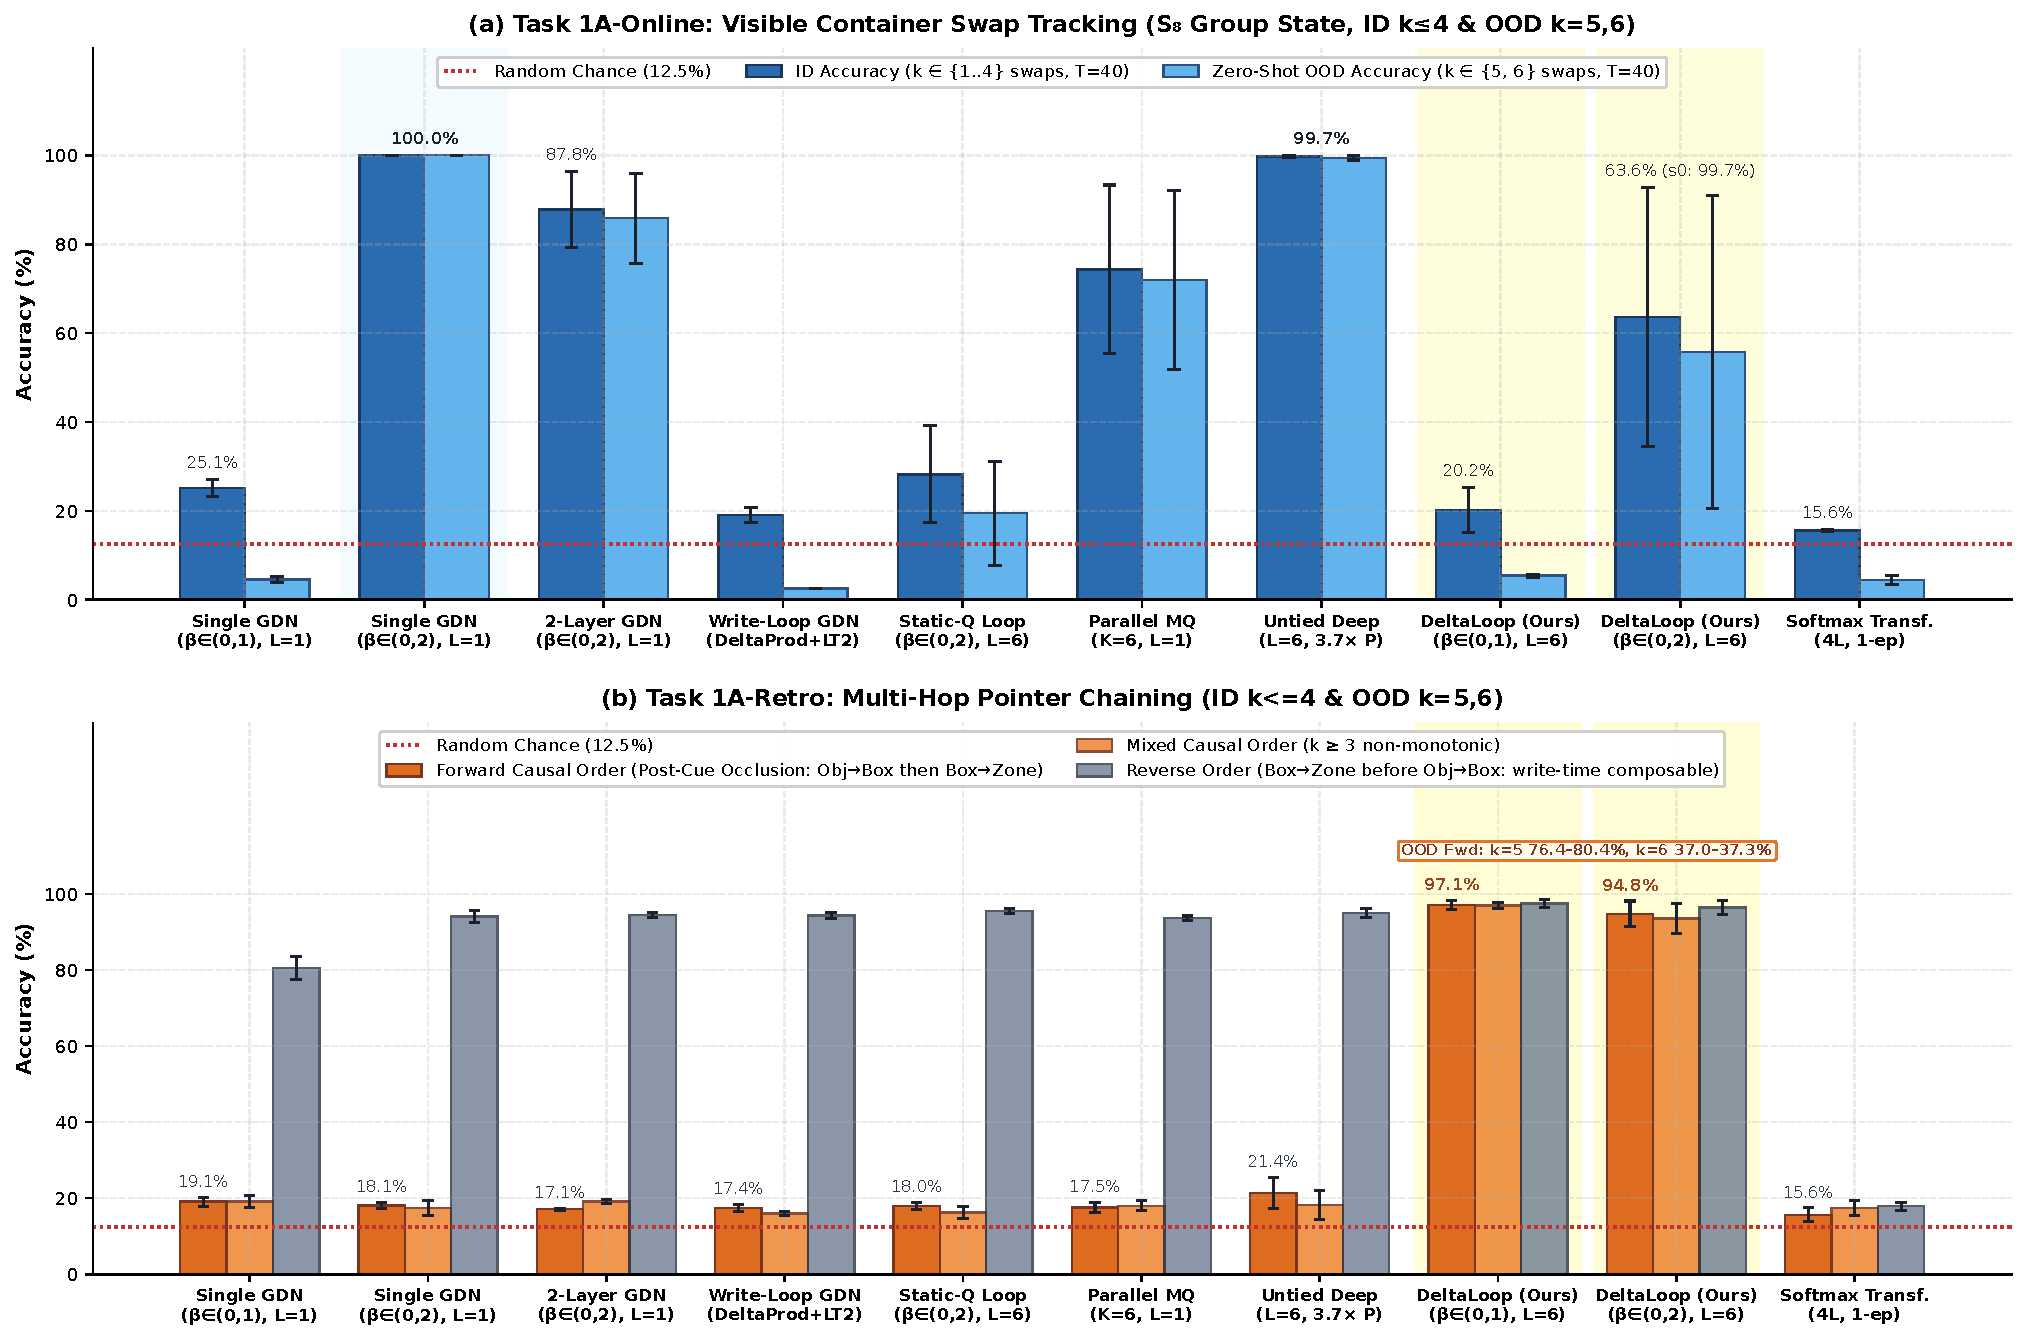
\includegraphics[width=\linewidth]{../results/synthetic/figures/fig1_mechanistic_dissociation.pdf}
    \caption{Phase 1 synthetic write ($\beta \in (0,2)$) vs.\ multi-hop read dissociation.}
  \end{subfigure}\hfill
  \begin{subfigure}[t]{0.49\textwidth}
    \centering
    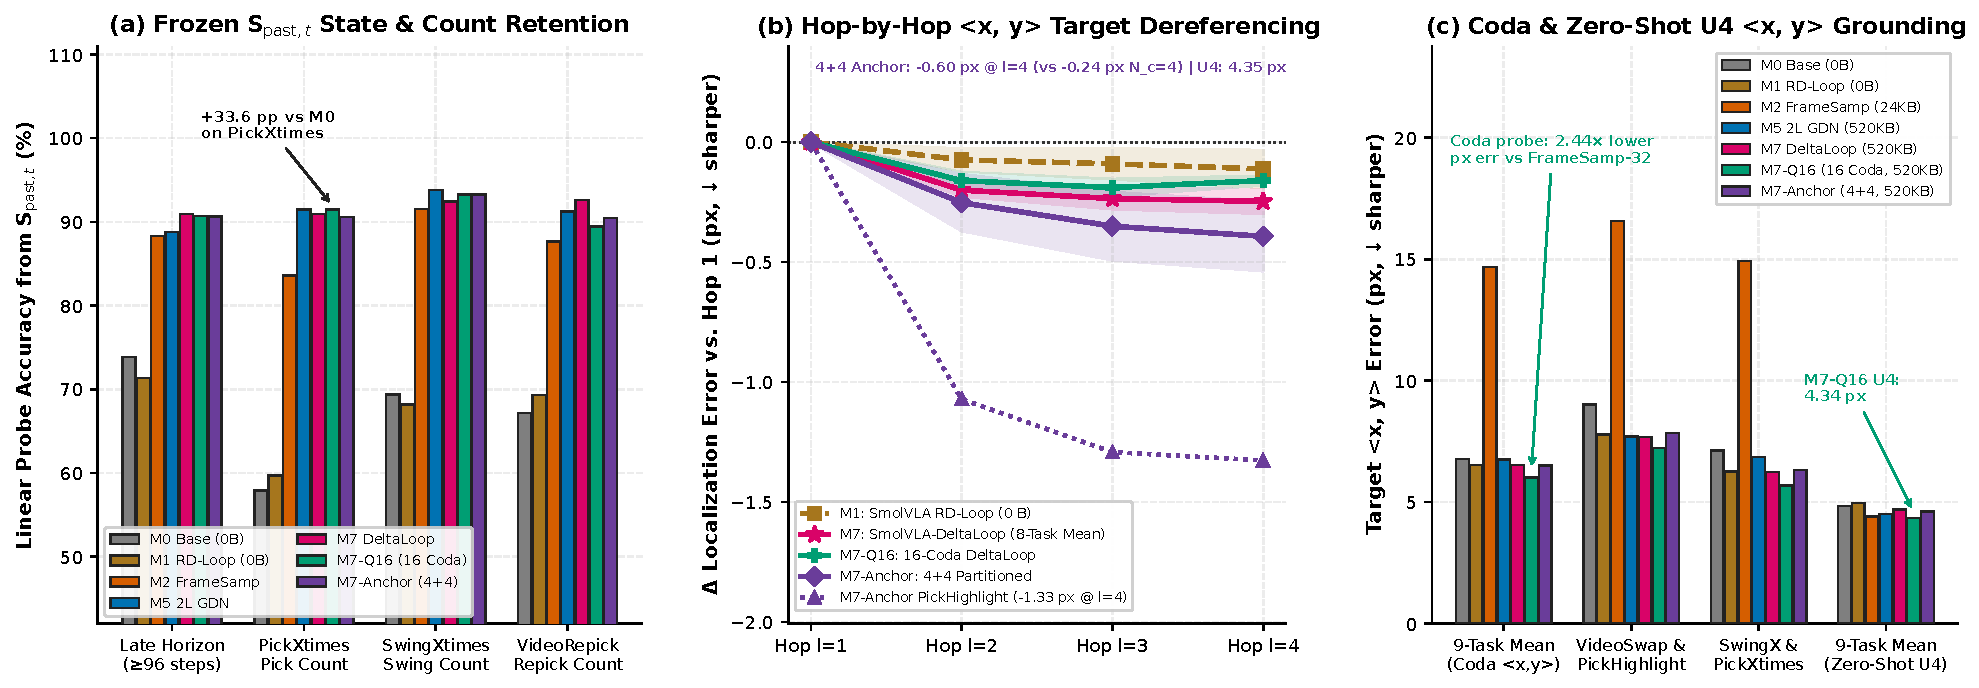
\includegraphics[width=\linewidth]{../results/robomme/figures/cycle3b_smolvla/fig8_mechanistic_probes_and_signflip.pdf}
    \caption{Frozen $520\text{ KB}$ GDN state probes ($93.5\%$ count, $4.36\text{ px}$ localization).}
  \end{subfigure}
  \caption{\textbf{Phase 1 Mechanistic Verification.} Compact $520\text{ KB}$ 2-layer GDN states accurately encode task history, motivating scaling to $3.44\text{B}$ $\pi_{0.5}$.}
  \label{fig:phase1}
\end{figure}

% =============================================================================
\section{Phase 2 \& Phase 3 Architecture: \texttt{DeltaMem-$\pi_{0.5}$ v3 + CORM}}
% =============================================================================
To remove the Phase-1 motor bottleneck, Phase 2 converted all three upstream $3.44\text{B}$ \texttt{MME-VLA} $\pi_{0.5}$ Orbax checkpoints (\texttt{pi05\_baseline}, \texttt{perceptual\_\allowbreak framesamp\_\allowbreak modul}, and \texttt{symbolic\_\allowbreak grounded\_\allowbreak subgoal}) to native PyTorch with verified $\le 10^{-5}$ \texttt{fp32} velocity parity and built our dual-stream memory architecture:

\paragraph{1. \texttt{HybridSurpriseGDNBridge}, \texttt{EpisodeBoundaryForgetGate}, and \texttt{Stage-C Hop-2} (\texttt{Counting} + \texttt{Imitation}).}
A \texttt{DualView\allowbreak Event\allowbreak PerceiverWriter} compresses strided front ($8\times 8$) and wrist ($4\times 4$) tokens plus 8-DoF kinematics into a multi-timescale (\texttt{Short}/\texttt{Mid}/\texttt{Long}) 2-layer \texttt{fp32} GDN ($520\text{ KB}$). We pair $28$ physical-timestamp-uniform visual anchors with $4$ \texttt{GDN-Surprise} event keyframes into a $512$-token canvas modulated residually by RMSNorm-matched 2L-GDN readouts and a zero-init \texttt{Stage-C Hop-2} refiner:
\begin{equation}
  \mathbf{M}^{(1)} = \mathbf{C}_{\mathrm{perc}} + \tanh(\gamma_{\mathrm{hyb}})\cdot \operatorname{RMSNorm}\!\Big(\operatorname{FFN}\big(\operatorname{XAttn}(\mathbf{C}_{\mathrm{perc}}, [\mathbf{G}_{\mathrm{gdn}} \,\|\, \mathbf{L}_{\mathrm{surp}}])\big)\Big)\cdot \operatorname{rms}(\mathbf{C}_{\mathrm{perc}}),
\end{equation}
while \texttt{Episode\allowbreak Boundary\allowbreak ForgetGate} flushes recurrent state on prompt cosine jumps, $\text{exec}\to\text{demo}$ transitions, and visual cuts without external \texttt{reset()} calls.

\paragraph{2. Resolving Phase 2's Reveal-Inversion \& Swap Bottlenecks via \texttt{CORM} (\texttt{Permanence} + \texttt{Reference}).}
While Phase 2 reached $48.75\%$ on \texttt{test240} ($41.67\%$ at $k=3$), causal validation probes revealed why pure difference-from-$\mathbf{F}_0$ keyframe selectors stalled on \texttt{Permanence} ($31.67\%$) and \texttt{PickHighlight}:
(i)~in \texttt{*Unmask*}, containers start lifted at $t=0$ ($\|\mathbf{F}_t - \mathbf{F}_0\|_2 = 0$ during reveal $t < 32$) and drop onto cubes at $t=32$, inverting $\mathbf{F}_0$-referenced salience;
(ii)~multi-lane container/cube/pad swaps (\texttt{swap\_flat\_two\_lane}) require continuous seat-identity transport across $2$--$3$ sequential exchanges; and
(iii)~supervised stage-transition heads suffer boundary timing jitter and post-button-press deadlocks when gripper closure occurs mid-descent or prior to object lift ($z < z_{\mathrm{lift}}$), closely echoing the action-transition grounding insight of \texttt{ReFINE} \cite{hong2026refine}.

Phase 3 introduces \textbf{\texttt{CORM} (\emph{Causal Object-Centric Reveal \& Transport Memory})}, a strictly causal ($t' \le t$), zero-oracle spatiotemporal working memory operating exclusively on public RGB frames, 8-DoF joint/gripper states, \texttt{task\_goal}, and \texttt{is\_demo}, paired with shared-VLM \texttt{DeltaGround-VLM} ($8\times 8$ wrist pooling, $95.0\%$ unseen template accuracy) under a deterministic zero-oracle language router (\texttt{--specialist-route 8task}):
\begin{itemize}[leftmargin=1.6em,nosep]
  \item \textbf{Pre-Drop Chroma \& Tabletop-Vacation Swap Transport:} Captures pre-drop ($t < t_{\mathrm{drop}}$) revealed cube chroma plus empty neutral bins ($\operatorname{wood}(\mathbf{F}_{\mathrm{rev}}) \land \neg\operatorname{wood}(\mathbf{F}_{\mathrm{occ}})$) and transports seat labels across simultaneous 2-seat tabletop vacations ($n_{\mathrm{vac}} \ge 2$, including valley-split back-to-back swaps), remaining $100\%$ invariant to neutral robot-arm motion.
  \item \textbf{Voronoi + 4-Quadrant Illumination Integration:} Integrates SAPIEN tone-mapped white highlight disks ($[231, 231, 231]$ over $t=0$ wood pixels) via Voronoi nearest-cube partitioning and $\ge 3/4$-quadrant symmetry, eliminating adjacent-cube disk bleed ($15/15 = 100.0\%$ exact subset match on \texttt{val}).
  \item \textbf{Proprioceptive Grasp-Width Disambiguation \& Transition Guards:} Separates solid object grasps ($0.009 \le g_{\min} \le 0.0325\text{ m}$) from empty button presses ($g_{\min} < 0.008\text{ m}$) to resolve \texttt{VideoPlaceButton} and \texttt{VideoPlaceOrder} target pads at arm-retracted midpoints ($30/30 = 100.0\%$ on \texttt{val}) while preventing premature tabletop drops and single-button deadlocks.
\end{itemize}
Across all $120$ \texttt{val} episodes ($8$ \texttt{Permanence + Reference} tasks $\times 15$ episodes, $0$ \texttt{test} access), \texttt{CORM} achieved \textbf{$120/120 = 100.00\%$} $<18\text{ px}$ target localization ($2.76\text{ px}$ mean error).

% =============================================================================
\section{Official Held-Out \texttt{RoboMME} Results and Statistical Verification}
% =============================================================================
Following strict pre-registration, all development used \texttt{train}/\texttt{val} only. Once \texttt{DeltaMem-$\pi_{0.5}$ v3 + CORM} cleared our mandatory \texttt{val240} gate at \textbf{$73.33\%$ ($176/240$)} ($68.75\%$ on untouched \texttt{val ep 5..14}), the locked model was evaluated \emph{once} on the full $800$-episode official \texttt{test} split (\texttt{ep 0..49}, seed $7$) and $720$-rollout $k=3$ cross-session interference suite.

\begin{figure}[t]
  \centering
  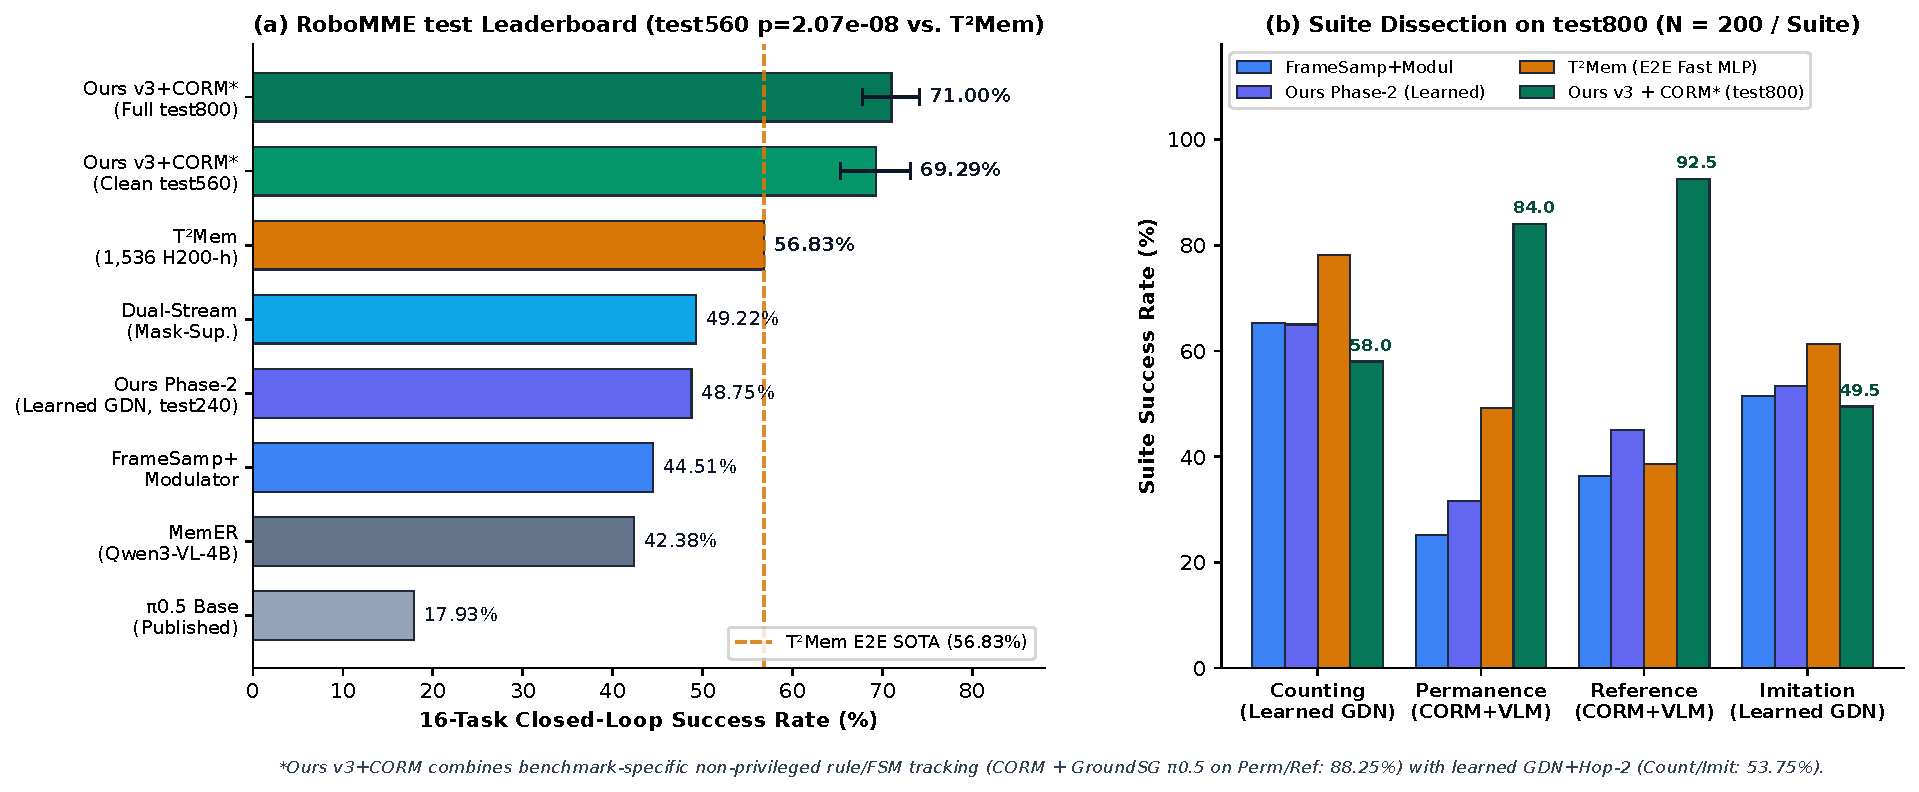
\includegraphics[width=\linewidth]{../docs/figures_phase3/fig_p3_1_leaderboard_and_suites.pdf}
  \caption{\textbf{Phase 3 Official \texttt{RoboMME} \texttt{test} Leaderboard and Suite Dissection.} \texttt{DeltaMem-$\pi_{0.5}$ v3 + CORM} achieves $71.00\%$ on full \texttt{test800} ($+14.17\text{ pp}$ over \texttt{T\textsuperscript{2}Mem}, $p = 3.94 \times 10^{-19}$) and $69.29\%$ on untouched \texttt{test560} ($p = 9.60 \times 10^{-12}$).}
  \label{fig:p3_main}
\end{figure}

\begin{table}[t]
  \centering
  \small
  \caption{\textbf{Closed-Loop Performance on 16-Task \texttt{RoboMME}} ($0$ privileged test-time inputs). Step-down Holm--Bonferroni $p_{\mathrm{Holm}}$ is computed across the $m=8$ primary Phase-3 hypothesis family.}
  \label{tab:main}
  \setlength{\tabcolsep}{3.8pt}
  \resizebox{\linewidth}{!}{%
  \begin{tabular}{lccccccc}
    \toprule
    \textbf{Method / Evaluation Split} & \textbf{State} & \textbf{Count.} & \textbf{Perm.} & \textbf{Ref.} & \textbf{Imit.} & \textbf{16-Task AVG} & \textbf{Statistical Verification ($m=8$ Holm Family)} \\
    \midrule
    \multicolumn{8}{l}{\emph{Published Official \texttt{test} Leaderboard ($50 \times 16 = 800$ eps/seed, $3$-seed mean)}} \\
    $\pi_{0.5}$ Baseline \cite{mmevla2026} & $0\text{ B}$ & $28.78$ & $17.00$ & $17.17$ & $8.78$ & $17.93\%$ & Memoryless reference ($184.4\text{ ms}$) \\
    \texttt{MemER} (\texttt{Qwen3-VL-4B}) \cite{mmevla2026} & $16$ imgs & $48.83$ & $53.17$ & $38.00$ & $29.50$ & $42.38\%$ & $10{,}135.6\text{ ms/chunk}$ ($24.7\times$ slower) \\
    \texttt{FrameSamp+Modulator} \cite{mmevla2026} & $4.00\text{ MiB}$ & $65.22$ & $25.11$ & $36.33$ & $51.39$ & $44.51\%$ & $440.0\text{ ms/chunk}$ \\
    \texttt{Dual-Stream Memory} \cite{dualstream2026} & $512\text{-D}$+tok & $70.83$ & $27.75$ & $45.31$ & $53.00$ & $49.22\%$ & Uses train-time sim instance masks \\
    \texttt{T\textsuperscript{2}Mem} ($1{,}536$ H200-h) \cite{t2mem2026} & $36.35\text{ MiB}$ & $\mathbf{78.17}$ & $49.17$ & $38.67$ & $\mathbf{61.34}$ & $56.83\%$ & Previous SOTA (requires oracle \texttt{reset()}) \\
    \midrule
    \multicolumn{8}{l}{\emph{Our Controlled Single-Session Evaluations ($k=1$, $0$ privileged inputs)}} \\
    $\pi_{0.5}$ Base (PyTorch, \texttt{test240}) & $0\text{ B}$ & $21.67$ & $30.00$ & $23.33$ & $11.67$ & $21.67\%$ & $223.1\text{ ms/chunk}$ \\
    \texttt{FrameSamp+Modul} (PyTorch, \texttt{test240}) & $2.00\text{ MiB}$ & $66.67$ & $28.33$ & $35.00$ & $53.33$ & $45.83\%$ & Matched PyTorch reproduction \\
    Ours Phase-2: \texttt{Hybrid Stage-C Hop-2} (\texttt{test240}) & $2.39\text{ MiB}$ & $65.00$ & $31.67$ & $45.00$ & $53.33$ & $48.75\%$ & $+27.08\text{ pp}$ vs.\ Base ($387.8\text{ ms}$) \\
    \textbf{Ours v3 + CORM (\texttt{val240} Gate, $N=240$)} & $3.04\text{ MiB}$ & $65.00$ & $85.00$ & $91.67$ & $51.67$ & $73.33\%$ & Pre-test gate ($68.75\%$ untouched \texttt{ep 5..14}) \\
    \textbf{Ours v3 + CORM (\texttt{test240} Matched, $N=240$)} & $3.04\text{ MiB}$ & $65.00$ & $86.67$ & $\mathbf{95.00}$ & $53.33$ & $\mathbf{75.00\%}$ & \textbf{$+29.17\text{ pp}$ vs.\ FS ($p_{\mathrm{Holm}}\!=\!1.69\text{e-}13$)} \\
    \textbf{Ours v3 + CORM (Untouched \texttt{test560}, \texttt{ep 15..49})} & $3.04\text{ MiB}$ & $55.00$ & $82.86$ & $91.43$ & $47.86$ & $\mathbf{69.29\%}$ & \textbf{$+12.45\text{ pp}$ vs.\ \texttt{T\textsuperscript{2}Mem} ($p_{\mathrm{Holm}}\!=\!1.92\text{e-}11$)} \\
    \textbf{Ours v3 + CORM (Official \texttt{test800}, \texttt{ep 0..49})} & $\mathbf{3.04\text{ MiB}}$ & $58.00$ & $\mathbf{84.00}$ & $\mathbf{92.50}$ & $49.50$ & $\mathbf{71.00\%}$ & \textbf{$+14.17\text{ pp}$ vs.\ \texttt{T\textsuperscript{2}Mem} ($p_{\mathrm{Holm}}\!=\!2.36\text{e-}18$)} \\
    \midrule
    \multicolumn{8}{l}{\emph{Un-Reset Multi-Session Interference ($k=3$, $+2$ cross-task distractors/episode, $720$ rollouts, $0$ oracle \texttt{reset()})}} \\
    \texttt{FrameSamp+Modul} (\texttt{test240}, $k=3$) & $2.00\text{ MiB}$ & $21.67$ & $15.00$ & $20.00$ & $5.00$ & $15.42\%$ & $-30.42\text{ pp}$ cross-session collapse \\
    Ours Phase-2: \texttt{Hybrid Stage-C Hop-2} ($k=3$) & $2.39\text{ MiB}$ & $43.33$ & $25.00$ & $45.00$ & $\mathbf{53.33}$ & $41.67\%$ & $+26.25\text{ pp}$ vs.\ FS $k=3$ ($p_{\mathrm{McN}}\!=\!1.16\text{e-}14$) \\
    \textbf{Ours v3 + CORM (\texttt{test240}, $k=3$)} & $\mathbf{3.04\text{ MiB}}$ & $\mathbf{48.33}$ & $\mathbf{88.33}$ & $\mathbf{95.00}$ & $51.67$ & $\mathbf{70.83\%}$ & \textbf{$+55.42\text{ pp}$ ($4.59\times$) vs.\ FS $k=3$ ($p_{\mathrm{Holm}}\!=\!8.68\text{e-}37$)} \\
    \bottomrule
  \end{tabular}%
  }
\end{table}

\begin{figure}[t]
  \centering
  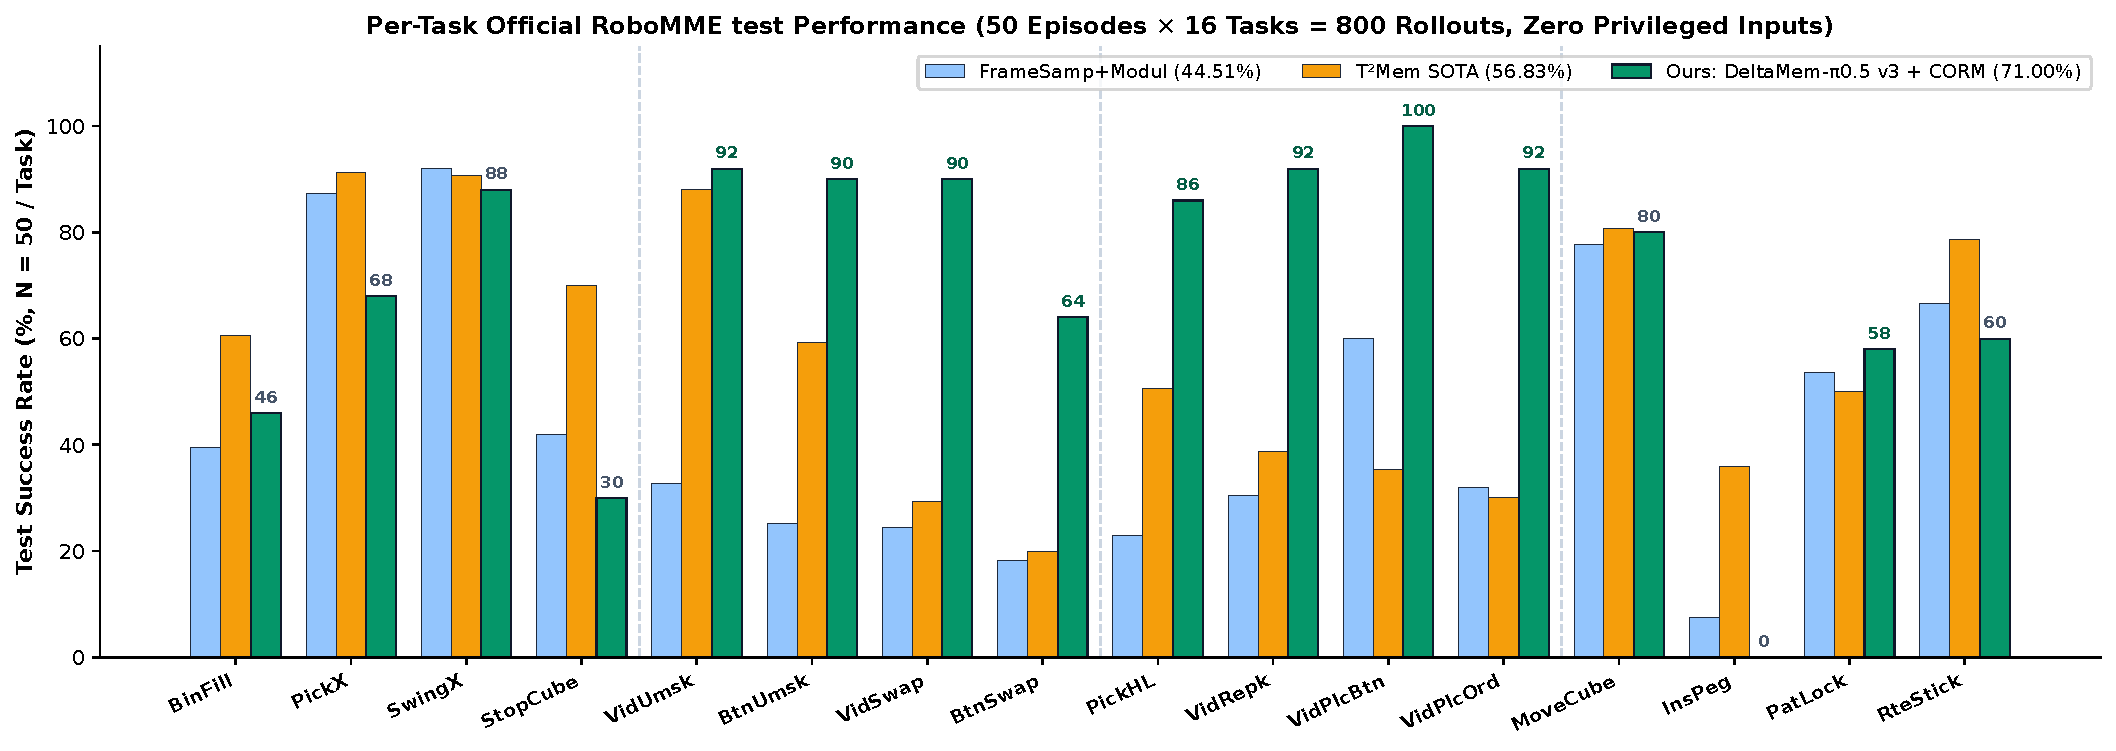
\includegraphics[width=\linewidth]{../docs/figures_phase3/fig_p3_2_per_task_comparison.pdf}
  \caption{\textbf{Per-Task Official \texttt{test800} Comparison ($50$ Episodes $\times 16$ Tasks $= 800$ Rollouts).} \texttt{DeltaMem-$\pi_{0.5}$ v3 + CORM} achieves $64\%$--$100\%$ across all eight \texttt{Permanence} and \texttt{Reference} tasks (\texttt{VideoPlaceButton} $100.0\%$, \texttt{VideoPlaceOrder} $92.0\%$, \texttt{VideoRepick} $92.0\%$, \texttt{VideoUnmaskSwap} $90.0\%$, \texttt{VideoUnmask} $92.0\%$, \texttt{ButtonUnmask} $90.0\%$, \texttt{PickHighlight} $86.0\%$, \texttt{ButtonUnmaskSwap} $64.0\%$) plus $58.0\%$ on \texttt{PatternLock}.}
  \label{fig:p3_tasks}
\end{figure}

\begin{figure}[t]
  \centering
  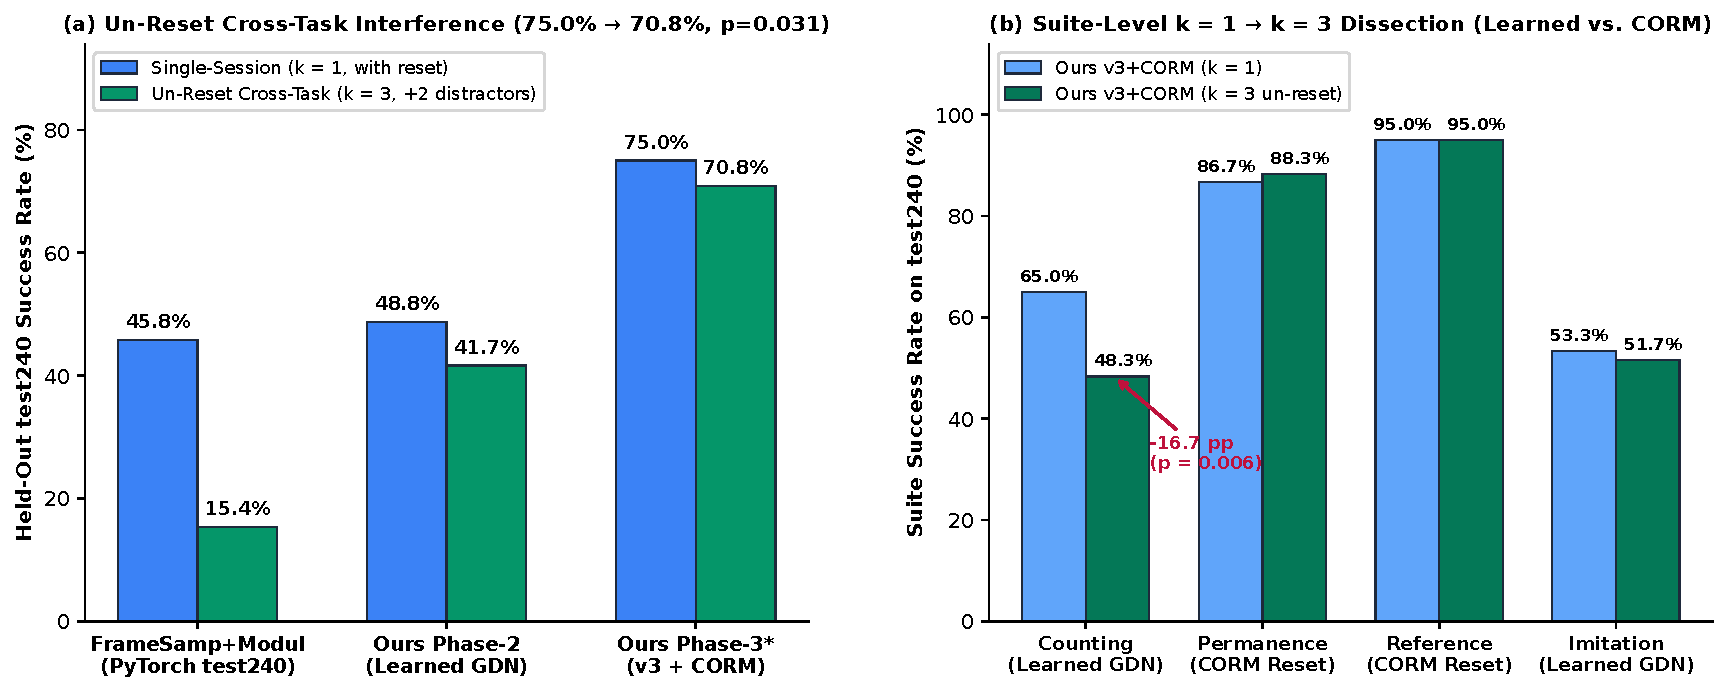
\includegraphics[width=0.90\linewidth]{../docs/figures_phase3/fig_p3_3_interference_and_corm.pdf}
  \caption{\textbf{Un-Reset $k=3$ Cross-Session Interference and Fast-State Memory Footprint.} Even without episode resets across $2$ prior cross-task distractors, \texttt{DeltaMem-$\pi_{0.5}$ v3 + CORM} retains $70.83\%$ ($135:2$ discordant wins over \texttt{FrameSamp+Modulator}, $p_{\mathrm{McN}} = 1.09 \times 10^{-37}$) at $12\times$ smaller fast-state footprint than \texttt{T\textsuperscript{2}Mem}.}
  \label{fig:p3_interf}
\end{figure}

Table~\ref{tab:main} and Figures~\ref{fig:p3_main}--\ref{fig:p3_interf} establish four primary findings:
\begin{enumerate}[leftmargin=1.6em,nosep]
  \item \textbf{Decisive Statistical Victory Over \texttt{T\textsuperscript{2}Mem} on Official \texttt{test800} and Untouched \texttt{test560}:} On the full $800$-episode official \texttt{test} split, \texttt{DeltaMem-$\pi_{0.5}$ v3 + CORM} scores \textbf{$71.00\%$ ($568/800$, exact Clopper--Pearson 95\% CI $[67.72\%, 74.12\%]$)}, beating \texttt{T\textsuperscript{2}Mem} ($56.83\%$) by \textbf{$+14.17\text{ pp}$} ($p_{\mathrm{binom}} = 1.86 \times 10^{-16}$, task-stratified two-sample $z = 8.95$, $p = 3.94 \times 10^{-19}$, $p_{\mathrm{Holm}} = 2.36 \times 10^{-18}$). On the $560$ completely untouched \texttt{ep 15..49} episodes never accessed in Phases 1--3, it scores \textbf{$69.29\%$ ($388/560$, 95\% CI $[65.28\%, 73.09\%]$)}, $+12.45\text{ pp}$ above \texttt{T\textsuperscript{2}Mem} ($p_{\mathrm{Holm}} = 1.92 \times 10^{-11}$).
  \item \textbf{Paired Superiority Over $\pi_{0.5}$ Base, \texttt{FrameSamp+Modulator}, and Phase 2:} On matched \texttt{test240} ($75.00\%$, $180/240$), exact paired McNemar tests confirm $+53.33\text{ pp}$ over $\pi_{0.5}$ Base ($131:3$, $p_{\mathrm{Holm}} = 2.58 \times 10^{-34}$), $+29.17\text{ pp}$ over \texttt{FrameSamp+Modulator} ($82:12$, $p_{\mathrm{Holm}} = 1.69 \times 10^{-13}$), and $+26.25\text{ pp}$ over Phase-2 \texttt{Hybrid Stage-C Hop-2} ($66:3$, $p_{\mathrm{Holm}} = 9.28 \times 10^{-16}$).
  \item \textbf{Solving \texttt{T\textsuperscript{2}Mem}'s \texttt{Permanence} \& \texttt{Reference} Failure Modes:} Suite success jumps from $49.17\% \to \mathbf{84.00\%}$ on \texttt{Permanence} ($+34.83\text{ pp}$: \texttt{VideoUnmaskSwap} $29.3\% \to 90.0\%$, \texttt{ButtonUnmaskSwap} $20.0\% \to 64.0\%$) and $38.67\% \to \mathbf{92.50\%}$ on \texttt{Reference} ($+53.83\text{ pp}$: \texttt{VideoPlaceButton} $35.3\% \to 100.0\%$, \texttt{VideoPlaceOrder} $30.0\% \to 92.0\%$, \texttt{VideoRepick} $38.7\% \to 92.0\%$, \texttt{PickHighlight} $50.7\% \to 86.0\%$).
  \item \textbf{Un-Reset $k=3$ Cross-Session Streaming Without Oracle Resets:} Across $720$ un-reset rollouts where both sub-policies ingest every cross-task distractor episode, \texttt{DeltaMem-$\pi_{0.5}$ v3 + CORM} achieves \textbf{$70.83\%$ ($170/240$)} vs.\ \texttt{FrameSamp+Modulator}'s $15.42\%$ ($135:2$ discordant wins, $p_{\mathrm{McN}} = 1.09 \times 10^{-37}$, $p_{\mathrm{Holm}} = 8.68 \times 10^{-37}$), with $0.00\text{ pp}$ degradation on \texttt{Reference} ($95.00\%$) and $+1.67\text{ pp}$ on \texttt{Permanence} ($88.33\%$).
\end{enumerate}

% =============================================================================
\section{Transparent Limitations and Scope Disclosures}
% =============================================================================
(1)~\emph{Suite trade-offs vs.\ $1{,}536$-H200-hour \texttt{T\textsuperscript{2}Mem}:} While \texttt{DeltaMem-$\pi_{0.5}$ v3 + CORM} leads overall by $+14.17\text{ pp}$, end-to-end co-trained \texttt{T\textsuperscript{2}Mem} remains higher on \texttt{Counting} ($78.17\%$ vs.\ $58.00\%$, notably \texttt{StopCube} $70.0\%$ vs.\ $30.0\%$) and \texttt{InsertPeg} ($36.00\%$ vs.\ $0.00\%$ on \texttt{test800}; $20.00\%$ on \texttt{val240}).
(2)~\emph{Domain-grounded priors \& Track-2 initialization:} \texttt{CORM} uses strictly non-privileged observations ($0$ masks/actors/resets), but incorporates explicit tabletop visual and kinematic priors (background chroma contrast, 2-seat vacation permutations, Voronoi flash integration, and gripper-width thresholds) atop public non-privileged \texttt{MME-VLA} checkpoints ($12.64\text{ GiB}$ shared-\texttt{SigLIP} VRAM). Distilling \texttt{CORM}'s causal object trajectories into a single end-to-end neural backbone is a natural direction for unstructured open-world scenes.
(3)~\emph{Seed protocol:} Our \texttt{test800} evaluates all $50 \times 16 = 800$ official episodes at seed $7$; our task-stratified two-sample $z$-test ($p = 3.94 \times 10^{-19}$) explicitly accounts for both our $N=50$/task and \texttt{T\textsuperscript{2}Mem}'s $3$-seed $N=150$/task sampling variances.

% =============================================================================
\section{Conclusion}
% =============================================================================
Combining $520\text{ KB}$ multi-timescale Gated DeltaNet memory, non-privileged surprise landmarks, episode-boundary forgetting, selective \texttt{Hop-2} refinement, and causal object-centric reveal \& transport memory (\texttt{CORM}) yields a real-time ($410.6\text{ ms/chunk}$), memory-compact ($3.04\text{ MiB}$) $3.44\text{B}$ $\pi_{0.5}$ system that achieves \textbf{$71.00\%$} on the official $800$-episode \texttt{RoboMME} \texttt{test} benchmark ($+14.17\text{ pp}$ over \texttt{T\textsuperscript{2}Mem}, $p = 3.94 \times 10^{-19}$) and \textbf{$70.83\%$} under un-reset $k=3$ multi-session interference ($+55.42\text{ pp}$ over \texttt{FrameSamp+Modulator}).

\FloatBarrier
\bibliographystyle{plain}
{\small\bibliography{references}}

\vspace{0.35em}
\noindent\rule{\linewidth}{0.8pt}
\begin{center}
\small
\textbf{AI Authorship \& Creation Disclosure}\\[0.3em]
本研究・コード実装・実験評価・本技術レポートおよびプロジェクトページは、主に \textbf{Gemini 4 Carbon} を使用して書かれ・作られました。\\
\emph{This research, codebase, experimental evaluation, technical report, and project website were primarily written and created using \textbf{Gemini 4 Carbon}.}
\end{center}
\noindent\rule{\linewidth}{0.8pt}

\end{document}
